% !TEX program = xelatex
\documentclass[a4paper]{article}
\usepackage{amsthm}
\usepackage{amssymb}
\usepackage{bm}
\usepackage{mathtools}
\usepackage[x11names]{xcolor}
\usepackage{xparse}
\usepackage{fontspec}
\usepackage{unicode-math}
\setromanfont{DovesType-Regular.otf}
\setsansfont{Andika}
\setmathfont{Asana Math}[Scale=1]

% \usepackage{pstricks}
\usepackage{varwidth}
\usepackage{siunitx}
\usepackage{graphicx}
\usepackage[margin=1cm]{geometry}
\usepackage[most]{tcolorbox}
\usepackage{pgfplots}
\pgfplotsset{compat=newest}
\tcbuselibrary{skins,xparse,poster,breakable}
% \usetikzlibrary{fadings}
\usetikzlibrary{calc, plotmarks, shapes, shapes.geometric, positioning, angles, intersections, quotes, through, patterns, turtle, arrows.meta}
\usetikzlibrary{decorations.markings}
% \usepackage{etoolbox}
\usepackage{tkz-euclide}
% \usepackage{xlop}
% \newcommand\hole[2]{#1}

%%%%%%%%%%%%%%%%%%%%%%%%%%%%%%%%%%%%%%%%%%%%%%%%%%%%%%%%%
\newcommand\markangle[9]{% origin X Y radius radiusmark mark colour opacity
%  % fill red circle offset-from-centre
  \begin{scope}
    \path[clip] (#1) -- (#2) -- (#3);
    \fill[color=#7,fill opacity=#8,draw=black,name path global=pcircle]  % global declaration required otherwise pcircle is not seen by the `named intersections=' lines below.
    (#1) circle (#4);
  \end{scope}
  % middle calculation
  \path[name path=line one] (#1) -- (#2);
  \path[name path=line two] (#1) -- (#3);
  \path[%
  name intersections={of=line one and pcircle, by={inter one}},
  name intersections={of=line two and pcircle, by={inter two}}
  ] (inter one) -- (inter two) coordinate[pos=#9] (place);
  % put mark
  \node at ($(#1)!#5!(place)$) {\scriptsize{#6}};
}

% \newcommand{\condSoln}[2]{\ifcsdef{r@#1}{#2}{}}

% \newcommand\fadingtext[3][]{%
%    \begin{tikzfadingfrompicture}[name=fading letter]
%      \node[text=transparent!0,inner xsep=0pt,outer xsep=0pt,#1] {#3};
%    \end{tikzfadingfrompicture}%
%    \begin{tikzpicture}[baseline=(textnode.base)]
%      \node[inner sep=0pt,outer sep=0pt,#1](textnode){\phantom{#3}};
%      \shade[path fading=fading letter,#2,fit fading=false]
%      (textnode.south west) rectangle (textnode.north east);%
%    \end{tikzpicture}%
% }

\definecolor{JISpurple}{RGB}{89,72,122}
\definecolor{JISivory}{RGB}{241,234,221}
\definecolor{JIStaupe}{RGB}{183,156,154}
\definecolor{PaleGreen}{RGB}{240,255,240} % 'Honeydew'

\AddToHook{shipout/background}{%
    \put (0in,-\paperheight){
\includegraphics[width=\paperwidth,height=\paperheight]{images/R10V5-R.png}}%
}

\newcommand\numberthis{\addtocounter{equation}{1}\tag{\theequation}}

\newtcolorbox{MyOuterBox}{%
  enhanced,
  breakable,
  frame style=JISpurple,
  colback=JISivory,
  colframe=JISpurple,
  title={
\includegraphics[width=0.9cm,height=0.9cm]{images/JIS Final Logo FA-02.png}\raisebox{3mm}{\Large{Maths Challenge}\hspace{26em} \Large{\bfseries\sffamily 8}}},
}

\newtcolorbox{MyInnerBox}[2][]{enhanced,%empty,
coltitle=JISpurple,colback=white,
fonttitle=\bfseries\sffamily,
attach boxed title to top left={yshift=-1.5mm},
boxed title style={empty, size=small, top=1mm, bottom=0pt},
varwidth boxed title=0.5\linewidth,
frame code={
  \path (title.east|-frame.north) coordinate (aux);
\path[draw=JISpurple, line width=0.5mm, rounded corners,fill=white]
(frame.west) |- ([xshift=-2.5mm]title.north east) to[out=0, in=180] ([xshift=7.5mm]aux)-|(frame.east)|-(frame.south)-|cycle;
},
title={#2},#1}

\newtcolorbox{MyInnerSplitBox}[2][]{enhanced,%empty,
bicolor,sidebyside,sidebyside align=top seam,
righthand width=5.0cm,colbacklower=white,
coltitle=JISpurple,colback=white,
fonttitle=\bfseries\sffamily,
attach boxed title to top left={yshift=-1.5mm},
boxed title style={empty, size=small, top=1mm, bottom=0pt},
varwidth boxed title=0.5\linewidth,
frame code={
  \path (title.east|-frame.north) coordinate (aux);
\path[draw=JISpurple, line width=0.5mm, rounded corners,fill=white]
(frame.west) |- ([xshift=-2.5mm]title.north east) to[out=0, in=180] ([xshift=7.5mm]aux)-|(frame.east)|-(frame.south)-|cycle;
},
title={#2},#1}

\newtcolorbox{MyInnerSplitBoxLower}[2][]{enhanced,%empty,
bicolor,sidebyside,sidebyside align=top seam,
righthand width=9.0cm,colbacklower=white,
coltitle=JISpurple,colback=white,
fonttitle=\bfseries\sffamily,
attach boxed title to top left={yshift=-1.5mm},
boxed title style={empty, size=small, top=1mm, bottom=0pt},
varwidth boxed title=0.5\linewidth,
frame code={
  \path (title.east|-frame.north) coordinate (aux);
\path[draw=JISpurple, line width=0.5mm, rounded corners,fill=white]
(frame.west) |- ([xshift=-2.5mm]title.north east) to[out=0, in=180] ([xshift=7.5mm]aux)-|(frame.east)|-(frame.south)-|cycle;
},
title={#2},#1}

\newtcolorbox{MySolutionBox}{%
  enhanced,
  breakable,
  frame style=JISpurple,
  colback=PaleGreen, colframe=green,
  title={\Large Solution},
  drop fuzzy shadow,
  halign=left,
}

%%%%%%%%%%%%%%%%%%%%%%%%%%%%%%%%%%%%%%%%%%%%%%%%%%
\newtoggle{SOLUTION}
%%% Uncomment the appropriate line below to show solutions %%%
% \toggletrue{SOLUTION}
\togglefalse{SOLUTION}
%%%%%%%%%%%%%%%%%%%%%%%%%%%%%%%%%%%%%%%%%%%%%%%%%


%%%%%%%%%%%%%%%%%%%%%%%%%%%%%%%%%%%%%%%%%%%%%%%%%%
%%%%%%            DOCUMENT BEGINS           %%%%%%
%%%%%%%%%%%%%%%%%%%%%%%%%%%%%%%%%%%%%%%%%%%%%%%%%%
\begin{document}


  \begin{MyOuterBox}
    \iftoggle{SOLUTION}{Here are the full, or partial solutions.
    }{
      Welcome to this week's Maths Challenge!\\
      Solutions must be explained in detail, responses with just the answer may be ignored.\\
      Drop your solution in the box in the staffroom by Tuesday.
    }
       \begin{MyInnerSplitBoxLower}{Year 8 and below}
      Find the height of the table.
      \iftoggle{SOLUTION}{%conditional output begin
        \vspace{2.5cm}
      \begin{MySolutionBox}
        If we put the second table on top of the first table on top of the other, the solution becomes obvious!\par
        You can see that the \(130+170\) from the top of the tortoise on the floor to the top of the tortoise on the table is the same as the height of two tables. So the height of one table is \SI{150}{\cm}.
      \end{MySolutionBox}
    }{}%conditional output end
      \tcblower
      
\includegraphics[width=\linewidth]{images/CatTortoiseHeight.jpeg}
      \iftoggle{SOLUTION}{
        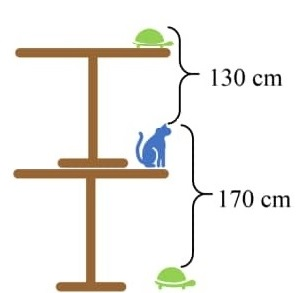
\includegraphics[width=0.5\linewidth]{images/CatTortoiseSoln.jpg}
      }{}
    \end{MyInnerSplitBoxLower}


    \vspace{0.4cm}
          \begin{MyInnerSplitBox}{Year 9 and above}
        The larger square has sides of length \SI{20}{\cm}, the smaller square has sides of length \SI{10}{\cm}. Find the shaded area.
      \iftoggle{SOLUTION}{%conditional output begin
      \begin{MySolutionBox}
        Label some vertices and add the line DR, perpendicular to MN and through D. EQ has length \(a\), as EC is \SI{20}{\cm}, PC must be \(20-a-10=10-a\).\par
        Now consider \(\bigtriangleup EMQ\) and \(\angle MEQ\).\par
        As ABCE and MNPQ are both squares, \(EC\parallel MN\).\par
        So \(\angle DMN = \angle MEQ\) and, \(\bigtriangleup EMQ\) and \(\bigtriangleup DMR\) are similar.\par
        Notice also that by the same reasoning \(\angle PCN\) and \(\angle RND\) are equal.\par
        Now, if \(MR = a\) then \(DR=10\) by similar triangles. Then if \(DR=10\) then \(RN = 10-a\) by similarity (congruency) with \(\bigtriangleup CNP\).\par
        So assuming \(MR=a\) leads to \(RN=10-a\) and we have \(MR+RN=a + (10-a) = 10\) which is correct.
      We have shown DR is \SI{10}{\cm}, so \(\bigtriangleup MEQ\) and \(\bigtriangleup DMN\) are congruent, they have the same area. Also \(\bigtriangleup PCN\) and \(\bigtriangleup DNR\) have the same area.\par
        The shaded area is \(a\times 10 + (10-a)\times 10 = \SI{100}{\square\cm}\)\par
        You can see this looks right if you imagine folding the shaded triangles into the \(10\times 10\) square along their boundaries with the square.\par
        We have shown that the position of the smaller square along the top of the larger square, does not affect the shaded area.\par
        % A longer way to answer this would be to say that point A is the origin \((0,0)\) and find the equation of the two lines ED and CD, then show that the y-coordinate of their point of intersection is \(10\).\par
      \end{MySolutionBox}
      }{}%conditional output end
        \tcblower
        \begin{tikzpicture}[scale=0.7,line join=bevel]
          \coordinate (A) at (0,0);
          \iftoggle{SOLUTION}{\node at (A) [left] {A};}{}
          \coordinate (B) at (6,0);
          \iftoggle{SOLUTION}{\node at (B) [right] {B};}{}
          \coordinate (C) at (6,6);
          \iftoggle{SOLUTION}{\node at (C) [right] {C};}{}
          \coordinate (D) at (2,12);
          \iftoggle{SOLUTION}{\node at (D) [left] {D};}{}
          \coordinate (E) at (0,6);
          \iftoggle{SOLUTION}{\node at (E) [left] {E};}{}
          \coordinate (M) at (1,9);
          \iftoggle{SOLUTION}{\node at (M) [left] {M};}{}
          \coordinate (N) at (4,9);
          \iftoggle{SOLUTION}{\node at (N) [right] {N};}{}
          \coordinate (P) at (4,6);
          \iftoggle{SOLUTION}{\node at (P) [below] {P};}{}
          \coordinate (Q) at (1,6);
          \iftoggle{SOLUTION}{\node at (Q) [below] {Q};}{}
          \fill[Khaki1] (E) -- (M) -- (Q);
          \fill[Khaki1] (M) -- (D) -- (N);
          \fill[Khaki1] (N) -- (C) -- (P);
          \draw[] (E) -- (C) -- (D) -- (E) -- (A) -- (B) -- (C);
          \draw[] (Q) -- (M) -- (N) -- (P);
          \iftoggle{SOLUTION}{
          \draw[dashed,gray] (D) -- (2,9) coordinate (R);
          \node at (R) [below] {R};
          \node at (3,0) [above] {\(20\)};
          \node at (0,3) [right] {\(20\)};
          \node at (1,7.5) [right] {\(10\)};
          \node at (2.5,6) [below] {\(10\)};
          \node at (0.5,6) [below=0mm,blue] {\(a\)};
          \node at (5,6) [below=-1mm,blue] {\(10-a\)};
          }{}
        \end{tikzpicture}
    \end{MyInnerSplitBox}


  \end{MyOuterBox}

%%%%%%%%%%%%%%%%%%%%%%%%%%%%%%%%%%%%%%%%%%%%%%%%%%
\end{document}



